% Inbuilt themes in beamer
\documentclass{beamer}

%packages:
% \usepackage{tfrupee}
% \usepackage{amsmath}
% \usepackage{amssymb}
% \usepackage{gensymb}
% \usepackage{txfonts}

% \def\inputGnumericTable{}

% \usepackage[latin1]{inputenc}                                 
% \usepackage{color}                                            
% \usepackage{array}                                            
% \usepackage{longtable}                                        
% \usepackage{calc}                                             
% \usepackage{multirow}                                         
% \usepackage{hhline}                                           
% \usepackage{ifthen}
% \usepackage{caption} 
% \captionsetup[table]{skip=3pt}  
% \providecommand{\pr}[1]{\ensuremath{\Pr\left(#1\right)}}
% \providecommand{\cbrak}[1]{\ensuremath{\left\{#1\right\}}}
% %\renewcommand{\thefigure}{\arabic{table}}
% \renewcommand{\thetable}{\arabic{table}}      

\setbeamertemplate{caption}[numbered]{}

\usepackage{enumitem}
\usepackage{tfrupee}
\usepackage{amsmath}
\usepackage{amssymb}
\usepackage{gensymb}
\usepackage{graphicx}
\usepackage{txfonts}

\def\inputGnumericTable{}

\usepackage[latin1]{inputenc}                                 
\usepackage{color}    
\usepackage{textcomp, gensymb}         
\usepackage{array}                                            
\usepackage{longtable}                                        
\usepackage{calc}                                             
\usepackage{multirow}                                         
\usepackage{hhline}                             
\usepackage{mathtools}
\usepackage{ifthen}
\usepackage{caption} 
\providecommand{\pr}[1]{\ensuremath{\Pr\left(#1\right)}}
\providecommand{\cbrak}[1]{\ensuremath{\left\{#1\right\}}}
\renewcommand{\thefigure}{\arabic{table}}
\renewcommand{\thetable}{\arabic{table}}   
\providecommand{\brak}[1]{\ensuremath{\left(#1\right)}}

% Theme choice:
\usetheme{CambridgeUS}

% Title page details: 
\title{AI1110 \\ Assignment-12} 
\author{Rajulapati Bhargava Ram \\ CS21BTECH11052}
\date{\today}
\logo{\large \LaTeX{}}


\begin{document}

% Title page frame
\begin{frame}
    \titlepage 
\end{frame}
\logo{}


% Outline frame
\begin{frame}{Outline}
    \tableofcontents
\end{frame}



\section{Question}
\begin{frame}{Question}
    \begin{block}{\textbf{Papoullis 10-8:} } 
      The input to a real system $H(\omega)$ is a WSS process $x(t)$ and the output equals $y(t)$. Show that if 
      \begin{align*}
         R_{xx}(\tau) = R_{yy}(\tau) \qquad  R_{xy}(-\tau) = -R_{xy}(\tau)
      \end{align*}   
      as in (10-130), then $H(\omega) = jB(\omega)$ where $B(\omega)$ is a function taking only the values $+1$ and $-1$.
      
      Special case: If $y(t) = \widehat{x}(t)$, then $B(\omega) = -sgn \;   \omega$        
     \end{block}
     
\end{frame}


\section{Theory}
\begin{frame}{Theory}
   \begin{block}{CORRELATION}
      The $\bf{Auto-correlation}$ of a process $x(t)$, real or complex, is by
      definition the mean of the product $x(t_1)x^*(t_2)$. Which is
     \begin{align}
       R_{xx}(t_1, t_2)  = E\cbrak{x(t_1)x^*(t_2)}
       				    &= R^*_{xx}(t_2, t_1)
     \end{align}
      The $\bf{Cross-correlation}$ of two process $x(t)$ and $y(t)$ is the function,
      \begin{align}
        R_{xy}(t_1, t_2)  = E\cbrak{x(t_1)y^*(t_2)}
       				    &= R^*_{yx}(t_2, t_1)
      \end{align}
   
  \end{block}   
  
	
\end{frame}

\begin{frame}{}
   \begin{block}{WIDE SENSE STATIONARY}
      A stochastic process $x(t)$ is called wide-sense stationary 
(abbreviated WSS) if its mean is constant 
      \begin{align}
        E\cbrak{x(t)} = \eta
	  \end{align} 
	  and its correlation depends only on $\tau=t_1 - t_2$:
	  \begin{align}
	    E\cbrak{x(t+\tau)x^*(t)} = R_{xx}(\tau)
      \end{align}
      	        
   \end{block}
   
   \begin{block}{}
     Two processes $x(t)$ and $y(t)$ are called jointly WSS if each is WSS and their cross-correlation depends only on $\tau = t_1 - t_2$: 
      \begin{align}
	     R_{xy}(\tau) = E\cbrak{x(t+\tau)y^*(t)}
      \end{align} 
      
   \end{block}
   
\end{frame}


\begin{frame}
   \begin{block}{THE POWER SPECTRUM}
      The power spectrum (or spectral density) of a WSS process $x(t)$, real 
or complex, is the Fourier transform $S(\omega)$ of its autocorrelation, $R_{xx}(\tau)=E\cbrak{x(t+\tau)x^*(t)}$:
	   \begin{align}
	      S_{xx}(\omega) = \int_{-\infty}^{\infty} R_{xx}(\tau)\; e^{-j\omega \tau} \, d\tau
	   \end{align}
	   
   \end{block}
   
   \begin{block}{}
   	  If $x(t)$ is a real process, then $R(\tau)$ is real and even; hence $S(\omega)$ is also real and even. In this case,
   	   \begin{align}
	      S_{xx}(\omega) = \int_{-\infty}^{\infty} R_{xx}(\tau)\; \cos \omega \tau \, d\tau
	   \end{align} 
	  From above we get, $S_{xx}(\omega)=S_{xx}(-\omega)$
	  
   \end{block}
\end{frame}

\begin{frame}
   \begin{block}{}
   	  The cross-power spectrum of two processes $x(t)$ and $y(t)$ is the Fourier transform $S_{xy}(\omega)$ of their cross-correlation $R_{xy}(\tau) = E\cbrak{x(t+\tau)y^*(t)}$:
   	  \begin{align}
   	  	S_{xy}(\omega) = \int_{-\infty}^{\infty} R_{xy}(\tau)\; e^{-j\omega \tau} \, d\tau 
   	  \end{align}
   \end{block}
   
   \begin{block}{}
   	  \begin{align}
   	  	 R_{xy}(\tau) = R_{xx}(\tau)\ast h^*(-\tau) \qquad R_{yy}(\tau) = R_{xy}(\tau)\ast h(\tau) \\
   	  	S_{xy}(\omega) = S_{xx}(\omega)H^*(\omega) \qquad S_{yy}(\omega) = S_{xy}(\omega)H(\omega)
   	  \end{align}
   	  Combining above equations we get,
   	  \begin{align}
   	  	R_{yy} = R_{xx}(\tau)\ast h^*(-\tau)\ast h(\tau)  
   	  	      &= R_{xx}(\tau)\ast \rho(\tau) \\
   	  	S_{yy}(\omega) = S_{xx}(\omega)H^*(\omega) H(\omega)
   	  	   			  &= S_{xx}(\omega) |H(\omega)|^2 \label{eq12}
   	  \end{align}
   	  Where $H(\omega)$ is called Transfer function.
   \end{block}
\end{frame}


\section{Solution}
\begin{frame}{Solution}
	In question given is,
	\begin{align}
		 R_{xx}(\tau) &= R_{yy}(\tau)  \label{eq13} \\
	     R_{xy}(-\tau) &= -R_{xy}(\tau) \label{eq14}
	\end{align}
	Begin with cross-power spectrum $S_{yy}(\omega)$,
	\begin{align}
	   S_{xy}(\omega) &= \int_{-\infty}^{\infty} R_{xy}(\tau)\; e^{-j\omega \tau} \, d\tau \\
	   S_{xy}(-\omega) &= \int_{-\infty}^{\infty} R_{xy}(\tau)\; e^{j\omega \tau} \, d\tau 
	\end{align}
	Replace $\tau$ with $-\tau$,
	\begin{align}
	   S_{xy}(-\omega) &= \int_{-\infty}^{\infty} R_{xy}(-\tau)\; e^{-j\omega \tau} \, d\tau 
	\end{align}
      
\end{frame}


\begin{frame}{}
    Using equation \eqref{eq14},
   \begin{align}
      S_{xy}(-\omega) &= \int_{-\infty}^{\infty} -R_{xy}(\tau)\; e^{-j\omega \tau} \, d\tau \\
      S_{xy}(-\omega) &= -\int_{-\infty}^{\infty} R_{xy}(\tau)\; e^{-j\omega \tau} \, d\tau \\
      S_{xy}(-\omega) &= -S_{xy}(\omega) 
   \end{align}
   Similarly using equation \eqref{eq13} we can get,
  \begin{align}
     S_{xx}(\omega)=S_{yy}(\omega)
  \end{align}
  Comparing above equation with equation \eqref{eq12} we get,
  \begin{align}
     |H(\omega)|^2 = 1
  \end{align}
         
\end{frame}
 

\begin{frame}{}
   Using equation (10),
   \begin{align}
      S_{xy}(-\omega) &= S_{xx}(-\omega)H^*(-\omega) \\
      -S_{xy}(\omega) &= S_{xx}(-\omega)H^*(-\omega)
   \end{align}  
     From equation (7) $S_{xx}(-\omega)=S_{xx}(\omega)$, So 
   \begin{align}
       -S_{xy}(\omega) &= S_{xx}(\omega)H^*(-\omega) \\
       \Rightarrow -H^*(\omega) &= H^*(-\omega) \\
       \Rightarrow H(-\omega) &= -H(\omega)
   \end{align}
    From above, the real part in $H(\omega)$ is zero, odd function and its in the form,
    \begin{align}
    		\therefore H(\omega) = j\:B(\omega)
    \end{align}
    Where $B(\omega)$ is a real function from equation (22),
    \begin{align}
    		\therefore |B(\omega)| = 1
    \end{align}
\end{frame}

\begin{frame}{}
	The graph of function $B(\omega)$,
	\begin{figure}[h!]
	  \centering 
	  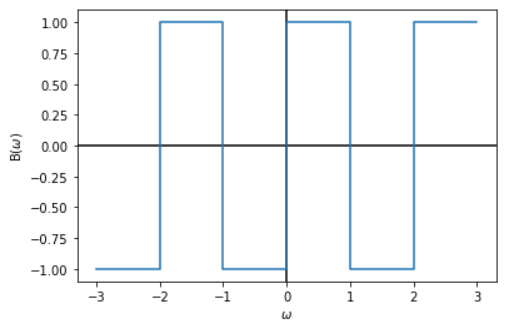
\includegraphics[]{./figs/plot.png}
	  \caption{}
	  \label{Fig1}
  \end{figure}
\end{frame}

\end{document}